\documentclass{article}
\usepackage[utf8]{inputenc}
\usepackage{graphicx}

\title{CIS 452-10 Lab 2}
\author{Thomas Bailey}
\date{January 2019}

\begin{document}

\maketitle

\begin{enumerate}
    \item Three lines are printed by the program: 'Before fork' and 'After fork' twice.
    
    \item The parent program begins execution. It prints out 'Before fork'. Then, the program forks. A child process is spawned, which is a duplicate of the parent. However, the child process starts on the command after the fork() happened. So, we see both the child and parent 'After fork' output.
    
    \item
    \begin{verbatim}
$ ps -l 17112
  F S   UID   PID  PPID  C PRI  NI ADDR SZ WCHAN  TTY        TIME CMD
  0 S  8977 17112 13704  0  80   0 -   574 hrtime pts/0      0:00 ./a.out
    \end{verbatim}

    From this output and the ps man page, I came up with the following information:
    \begin{enumerate}
        \item My effective user ID is 8977.
        \item The process ID is 17112.
        \item The parent's process ID is 13704.
        \item The process had 0 percent processor utilization.
        \item The process has a priority of 80. Lower numbers indicate higher priority.
        \item The 'nice' value of my process is 0. A nice program is kind to its program peers and doesn't monopolize the CPU.
        \item The physical size of the core image for the process is 574 bytes.
        \item The name of the kernel function in which the process is sleeping is called hrtime. The process is probably sleeping here because of the wait(10) call.
        \item The cumulative CPU time is 0:00, indicating the process was not very intensive.
        \item The command used to start the process was ./a.out.
    \end{enumerate}
    
    \item
    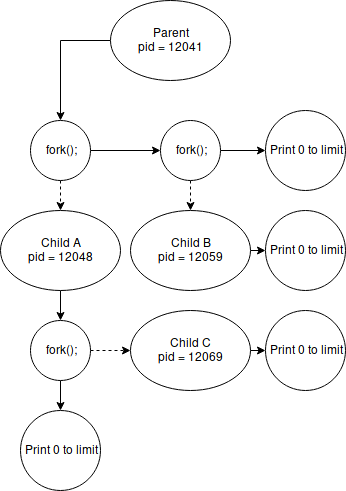
\includegraphics[scale=0.6]{index.png}
    
    \item I observed that the program prints the integers from 0 to limit four times in total. The output is not always the same, the loops sometimes being printed separately and sometimes concurrently. The concurrent loop happens because sometimes the parent processes are executing at the same time as their children.
    
    \item
    \begin{verbatim}
child = wait(&status);\end{verbatim}
    \item The child prints first  because the parent doesn't print until wait() returns.
    
    \item The two values that are printed out by the parent in sample program 3 are the process ID of the child, and the status code that was returned. When exit(n) is called with an integer n, n will correspond to a status code. Then, wait(\&s) will store the status code in the variable s. Wait returns the process ID of the child, which gets stored in child.
    
    \item The second print line ("After the exec") is \textbf{never} printed because it \textbf{DOESN'T EXIST}!!!1 The memory that contained that command was overwritten by the execvp() call.
    
    \item The second argument passed to execvp() is the location for the null terminated string containing the arguments for the file to be executed.
    
    
    
    
\end{enumerate}

\end{document}
